\chapter{非刚体和多刚体运动下的SfM技术}
\label{sec:non-rigid_SfM}
为了处理场景中的动态物体,一般将场景中不同运动物体进行分割,并对这些不同运动的物体分别进行三维重建是一个比较直接的方案。但考虑到所有物体的运动和三维信息同时都反应到了视频序列中,理论上这些物体的运动和三维信息可以同时进行求解\cite{Tomasi1992Shape}。在给定特征对应或者像素对应关系的基础上,基于矩阵分解的方式可以从表示了图像序列的特征矩阵中同时求解出动态物体的分割、恢复出各自物体的运动信息以及场景和物体的三维信息。如图\cite{zappella2013joint}所示,这些方法根据场景三维结构在相机运动的模型下生成图像序列的过程,推导出最终的特征矩阵的特性。根据不同物体运动不同在矩阵中反应出的不同性质,对矩阵进行重新组织,并可以根据图像序列的生成模型将每部分的矩阵分解乘包含了相机运动的矩阵乘以三维信息的形式,利用矩阵中提供的约束同时完成运动物体分割、运动求解以及三维信息恢复。

\begin{figure}[thbp]
	\centering
	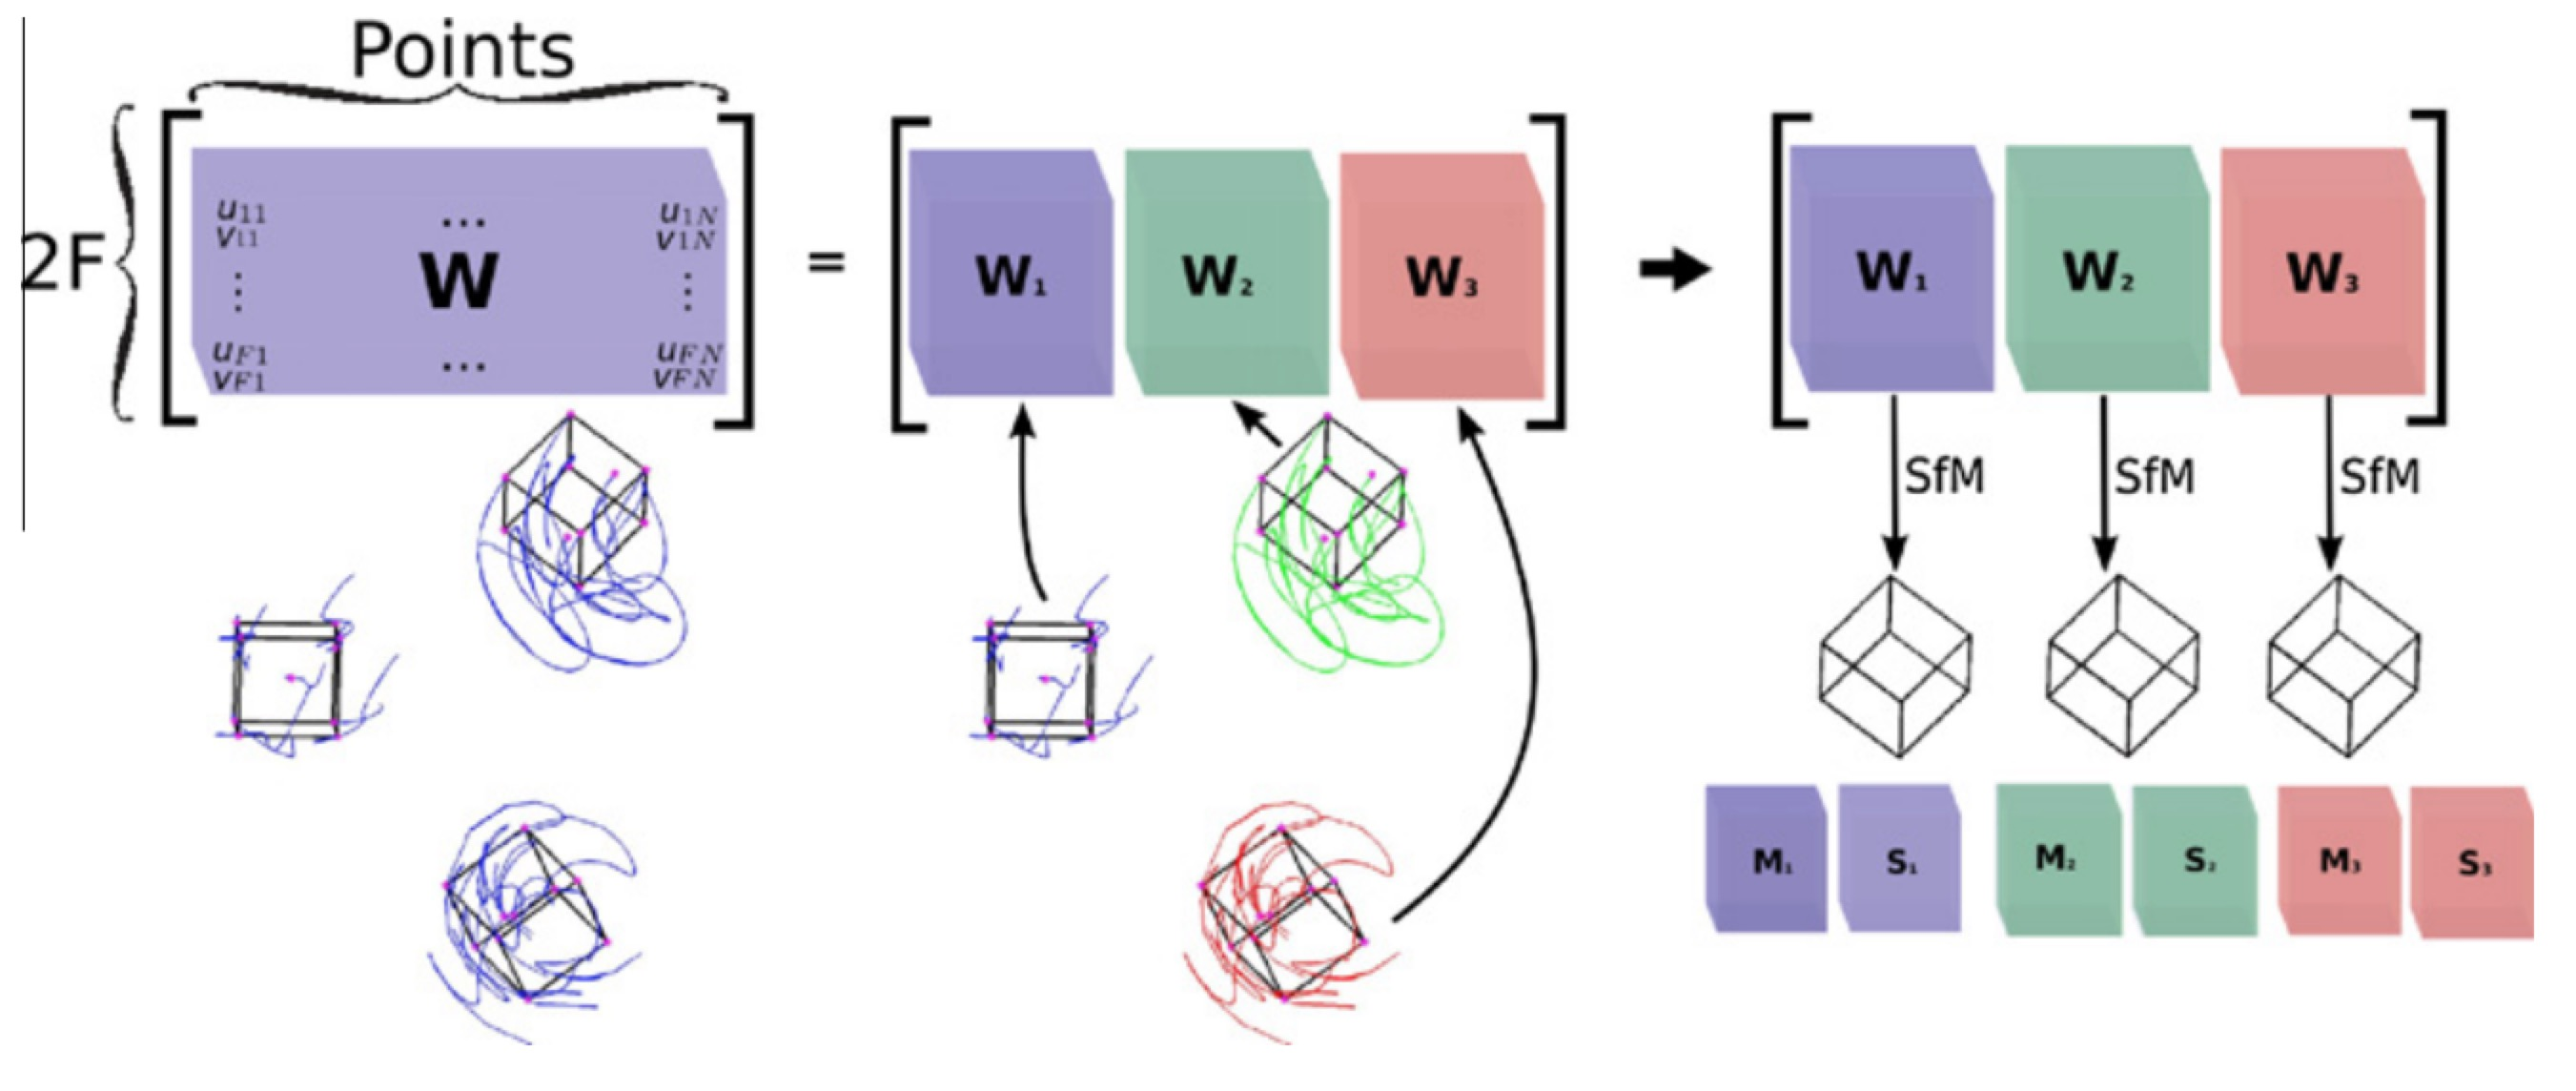
\includegraphics[width=0.9\textwidth]{figs/1-3/matrix.jpeg}
	\caption{多刚体下SfM矩阵可以拆解成各个子矩阵的组合来逐个单独求解~\cite{fox1999}。}
	\label{fig:rhino}
\end{figure}

\section{视频序列帧中特征变化的子空间约束}\label{subsec:subspace}
与一般对特征的处理相同,假如我们可以跟踪到视频序列中的一系列特征,比如使用光流等方法\cite{Fanani2016Keypoint},如图\ref{fig:feature_trajectory}所示。为了便于推导,我们在这里假设这些特征在1至f帧之间均连续观测到,噪声和缺失的情况会另外探讨。我们将观测到的特征点记做$x_{ij}=(u_{ij},v_{ij})$,其中下标中$i$代表第$i$帧,$j$代表第$j$个特征点。由于这些特征点是由相机在三维空间中运动生成的,所以这一系列特征点应当连续变化并与三维场景和相机运动对应。我们将这些特征点的坐标根据编号和时间序列排布到一个矩阵中,如式\eqref{eq:measurementMatrix}所示,纵坐标方向上按照帧的时间顺序排列,横坐标按照特征点的编号排列。

\begin{equation}\label{eq:measurementMatrix}
W=
\begin{pmatrix}
u_{11}& \cdots & u_{1p}\\
\vdots& \vdots &\vdots\\
u_{f1}& \cdots & u_{fp}\\
v_{11}& \cdots & v_{1p}\\
\vdots& \vdots &\vdots\\
v_{f1}& \cdots & v_{fp}
\end{pmatrix}
\end{equation}
矩阵分解方法认为这个矩阵是由相机的运动和三维结果矩阵合成而成,可以通过矩阵分解恢复出原始的信息。

\begin{figure}[htbp]
	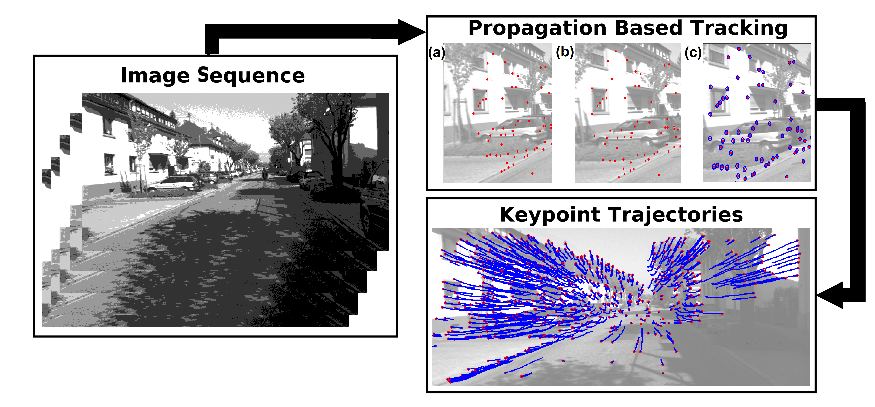
\includegraphics[width=1\textwidth]{figs/1-3/feature_trajectory.png} 
	\caption{跟踪得到的特征点序列轨迹\cite{Fanani2016Keypoint},观测矩阵是将图中连续出现的特征点坐标放到矩阵中,能够表示特征点在空间和时域上的关系。}
	\label{fig:feature_trajectory}
\end{figure}

通过矩阵分解的方式联合求解摄像机运动和三维信息,是SfM中一个重要的方法。这种方法具有优雅的数学描述,充分的考虑到了特征之间在空间和时间上的关联约束。这种方法最早由Tomasi和Kanade\cite{Tomasi1992Shape}根据秩理论在1992年提出。他们的理论指出,在一个面向静态场景的较短的序列中,包含了在整个帧序列上所有跟踪到的特征点的观测矩阵(measurement matrix),它的秩最多是4。特别的对欧式坐标系下的垂直投影来说秩最多是3\cite{Costeira1995A,Tomasi1992Shape,Irani2002Multi,Liu2011Subspace}。这种秩下的约束表明了这些特征点在时间变化是有明显关联的。
\section{观测矩阵与相机运动及三维结构的关系}\label{subsec:measurementMatrix}
观测矩阵是由相机的运动和三维点共通生成的,本节主要讲观测矩阵与这两个信息之间有什么样的关系。
由于垂直投影垂直投影形式较为简单,故我们先从垂直投影的情形来做说明\cite{Tomasi1992Shape}。垂直投影的形式如式\eqref{eq:orthogonalProjection}所示,是三维点的$x,y$分量的直接映射。
\begin{equation}\label{eq:orthogonalProjection}
x_j=
\begin{pmatrix}
R_{11} & R_{12} & R_{13} & t_1\\
R_{21} & R_{22} & R_{23} & t_2
\end{pmatrix}
\begin{pmatrix}
X_j\\Y_j\\Z_j\\1
\end{pmatrix}
\end{equation}
其中$R_{ij}$是旋转矩阵$R$的第$(i,j)$个元素,$t_i$是平移分量的元素,上述矩阵中仅包含了旋转矩阵的前两行,第三行可以用这两行的叉乘求得。$[X_j,Y_j,Z_j,1]$是第j个三维点齐次坐标,我们把第j个三维点的齐次坐标写作$X_j$,则对第n帧中的p个点来说,三维点的齐次坐标集合可以写作$[X_1,\cdots,X_p]\in \mathbb{R}^{4\times p}$。设$R_x^j$和$R_y^j$分别代表了第j帧姿态的旋转矩阵的第一行和第二行,$t_x^j$和$t_y^j$代表了第j帧姿态的平移分量。我们对每个相机对整个三维点集用式\eqref{eq:orthogonalProjection}进行投影,将得到的二维点堆叠起来就可以得到式\eqref{eq:measurementMatrix}中的观测矩阵,如式\eqref{eq:orthogonalMeasurementMatrix}所示。

\begin{equation}\label{eq:orthogonalMeasurementMatrix}
\begin{pmatrix}
u_{11}& \cdots & u_{1p}\\
\vdots& \vdots &\vdots\\
u_{f1}& \cdots & u_{fp}\\
v_{11}& \cdots & v_{1p}\\
\vdots& \vdots &\vdots\\
v_{f1}& \cdots & v_{fp}
\end{pmatrix}
=
\begin{pmatrix}
{R_x^1}^T & t_x^1\\
\vdots & \vdots\\
{R_x^f}^T & t_x^f\\
{R_y^1}^T & t_y^1\\
\vdots & \vdots\\
{R_y^f}^T & t_y^f\\
\end{pmatrix}
\begin{pmatrix}
X_1&\cdots &X_p
\end{pmatrix}
\end{equation}


一个更复杂的情况是在仿射相机(affine camera)的模型下进行推导\cite{Feng2013Joint}。在这个假设下,相机的投影模型可以简化成如式\eqref{eq:affineCameraModelProjection}所示的形式,旋转矩阵中最后一行为0。
\begin{equation}\label{eq:affineCameraModelProjection}
x_j=\pi
(
\begin{pmatrix}
f & 0 & c_1\\
0 & f& c_2\\
0 & 0 &1
\end{pmatrix}
\begin{pmatrix}
R_{11} & R_{12} & R_{13} & t_1\\
R_{21} & R_{22} & R_{23} & t_2\\
0      & 0      & 0      & d_0
\end{pmatrix}
\begin{pmatrix}
X_j\\Y_j\\Z_j\\1
\end{pmatrix}
)
\end{equation}
其中$f$是相机的焦距,$(c_1,c_2)$是图像中心,$d_0\in \mathbb{R}$ 是一个常量,$R_{ij}$是旋转矩阵$R$的第$(i,j)$个元素,$t_i$是平移分量的元素,$\pi(\cdot)$是讲齐次量变化为非齐次量的过程,即$\pi([X,Y,Z]=[X/Z,Y/Z])$。
我们定义如下的观测矩阵,其中每个位置为当前帧的二维位置减去第一帧的位置$x_{ij}-x_{1j}$。则对每一个三维点$X_j$来说这组观测矩阵元素可以写成式\eqref{eq:affineMearuement}。
\begin{eqnarray}\label{eq:affineMearuement}
\begin{pmatrix}
u_{ij}\\
v_{ij}
\end{pmatrix}
&=&
x_{ij}-x_{1j}\\
&=&\frac{f}{d_0}
\begin{pmatrix}
(R_{11}^i-1)X_{j}+R_{12}^i Y +R_{13}^i Z_j+t_x^i\\
R_{21}X_j + (R_{22}^i-1)Y_j+R_{23}^i Z_j+t_x^i
\end{pmatrix}
\end{eqnarray}
则显然的在仿射投影关系下,观测矩阵也是由包含姿态的矩阵乘以包含了三维点信息的矩阵得到。

对投影相机来说,上述的简单关系更复杂一些,因为齐次化过程依赖于每个像素的深度信息\cite{Sturm1996A}。考虑到齐次坐标到非齐次坐标的变换,为了能够通过矩阵分解的方式进行求解,我们把齐次化中的尺度因子作为一个需要先求解的参数进行处理。我们把投影关系下的尺度因子记做$\lambda\in \mathbb{R}$。我们记${P_i\in \mathbb{R}^{3\times4}}_{i=1}^f$ 是一系列相机的投影矩阵,包含了旋转和投影及内参的关系,把齐次坐标表示的三维点${X_j\in \mathbb{R}^4}_{j=1}^p$映射到第i个相机里,即满足投影关系$\lambda_{ij}x_{ij}=P_i X_j$。在整个视频序列以及整个三维点集上完整的投影投影过程如式\eqref{eq:projectiveMeasurementMatrix}所示,
\begin{equation}\label{eq:projectiveMeasurementMatrix}
W=
\begin{pmatrix}
\lambda_{11}x_{11}&\cdots&\lambda_{1p}x_{1p}\\
\vdots&\ddots & \vdots\\
\lambda_{f1}x_{f1}&\cdots&\lambda_{fp}x_{fp}
\end{pmatrix}
=
\begin{pmatrix}
P_1\\
\vdots\\
P_f
\end{pmatrix}
\begin{pmatrix}
X_1,&\cdots,&X_p
\end{pmatrix}.
\end{equation}

Sturm 和 Trigss\cite{Sturm1996A} 根据基本矩阵和极点的约束对式\eqref{eq:projectiveMeasurementMatrix}中的$\lambda$进行了求解。由于单目视频本来就无法恢复尺度,我们可以任意选择一个深度尺度,比如设$\lambda_{1p}=1$作为初始值。根据不同帧之间的极线约束,这些射影相机观测矩阵中的深度尺度可以按照式\eqref{eq:projectiveDepthUpdate}进行更新求解:
\begin{equation}\label{eq:projectiveDepthUpdate}
\lambda_{mp}=\frac{(e_{mn}\times x_{mp})\cdot(F_{mn}x_{np})}{\Vert e_{mn}\times x_{mp}\Vert}\lambda_{np}.
\end{equation} 
其中$m,n\in{1,2,\cdots,f}$,$F_{mn}$和$e_{mn}$分别为$m$对$n$帧之间定义的基本矩阵和极点。在求解得所有的深度尺度$\lambda_{mp}$之后我们就可以得到射影相机模型下的观测矩阵。

针对射影相机的另一个处理方式是Liu等人\cite{Feng2013Joint}所采用的小运动近似的方式。这种方式中假设在视频序列中相机的运动相对与帧率来说非常缓慢,每帧之间的旋转运动较小,可以使用李代数到旋转矩阵的一阶泰勒展开做为近似,在这个近似下线性关系更加明确,能够得到简单的观测矩阵。
\section{针对多刚体系统的观测矩阵分解}
我们先从静态世界或者整体就是一个刚体的系统进行考虑,通过\ref{subsec:subspace}节的方式,我们可以在一个视频序列中得到它的观测矩阵$W\in \mathbb{R^{2f\times p}}$,这里$f$是帧数$p$是三维点数。根据\ref{subsec:measurementMatrix}节中的推导,我们可以看出这个观测矩阵可以分解成运动矩阵$M\in \mathbb{R}^{2f\times 4}$和形状矩阵$S\in\mathbb{R}^{4\times p}$即如式\eqref{eq:Factorization}所示:
\begin{equation}\label{eq:Factorization}
W=M S .
\end{equation}

在求解过程中,我们在得到观测矩阵$W$之后,基于秩约束(Rank constraint)\cite{Costeira1998A},矩阵$W$可以用奇异值分解(SVD)进行分解,得到
\begin{equation}\label{eq:svdFactorization}
W=U\Sigma V,
\end{equation}
的形式。其中$\Sigma\in \mathbb{R}^{4\times4}$是一个对角阵,包含了最大的四个特征值,$U\in \mathbb{R}^{2f\times4}$和$V\in \mathbb{R}^{p\times4}$是对应到最大的四个特征值的特征向量。之后我们可以用$\hat{M}=U\Sigma^{1/2}$和$\hat{S}=\Sigma^{1/2}V^T$来表示运动矩阵和形状矩阵。但是式\eqref{eq:svdFactorization}中的分解并不是唯一的,真实的运动矩阵$M$和形状矩阵$S$还需要再找到一个映射矩阵$A$使得整个分解过程如下式所示:
\begin{equation}
W=M S=(\hat{M}A)(A^{-1}\hat{S}).
\end{equation}
其中矩阵$A$可以通过旋转矩阵和平移所带有的先验约束进行求解,并可以转化成一个最小二乘形式线性求解过程\cite{Costeira1998A,Tomasi1992Shape}。

上述就是通过分解形式联合求解静态场景问题的基本框架,这个框架可以比较容易的推广到场景中存在独立运动的多个刚体的情形\cite{Costeira1998A}。我们假设场景中包含了$n$个独立运动的刚体,则我们可以通过列交换的形式把观测矩阵$W$中的特征序列根据刚体分组成$[W_1,\cdots,W_n]$,这个过程可以用一个排列矩阵$\Gamma$来表示,如式\eqref{eq:multibodyMeasurementMatrix}所示,其中$\Gamma\in \mathbb{R}^{p\times p}$是一个未知的排列矩阵。
\begin{equation}\label{eq:multibodyMeasurementMatrix}
\bar{W}=W \Gamma=\begin{pmatrix}
W_1,\cdots,W_n
\end{pmatrix}
\end{equation}

在没有噪声的情况下,每一个独立的$W_i$即和前述静态场景中的观测矩阵等价应当在一个秩不超过4的子空间中。这样每个$W_i$可以进行单独的分解,得到该刚体的运动矩阵$M_i$以及形状矩阵$S_i$,如下式所示:
\begin{equation}\label{eq:multibodyFactorization}
\bar{W}=\bar{M} \bar{S} = 
\begin{pmatrix}
M_1,\cdots,M_n
\end{pmatrix}
\begin{pmatrix}
S_1 & &\\
&\ddots&\\
&      &S_n
\end{pmatrix}
.\end{equation}
这样对多刚体运动的问题来说,最关键的就是求解排列矩阵$\Gamma$让分解得到的矩阵$\bar{S}$具有块对角的性质。

多刚体运动恢复结构(Multibody Structure from Motion)对标准SfM下刚体相机的运动进行了拓展,变成了n个刚体的刚性运动模型。为了解决多刚体运动恢复结构问题,在仿射相机模型的假设下Costeira和Kanade\cite{Costeira1998A} 引入了一个形状交互矩阵的概念。这个理论里对物体形状构造了一个数学上的可证明的、对刚体运动具有不变性、不依赖于坐标系的描述。这里的结构交互矩阵被证明可以保持在原始子空间里的结构。我们设$\bar{W}=U\Sigma V^T$是一个秩r的观测矩阵SVD分解结果,其中$U\in \mathbb{R}^{2f\times r}$, $\Sigma\in \mathbb{R}^{r\times r}$,$V\in \mathbb{R}^{p\times r}$。则形状交互矩阵$Q$就可以定义为:
\begin{equation}\label{eq:shapeInteractionMatrix}
Q=VV^T\in \mathbb{R}^{p\times p}.
\end{equation}
式\eqref{eq:shapeInteractionMatrix}具有一个特殊的形状,当两个特征序列分别属于是两个刚体的时候,$Q$的元素会是0。 这个特性可以在数学上得到证明\cite{kanatani2001motionA}。 在这个理论基础上,矩阵分解的求解过程可以基于对$Q$的排序和元素大小的限制来或得不同刚体的分割以及三维信息的重建。
在\cite{Costeira1998A}中,这种运动刚体的分割和聚类是通过最大化式\eqref{eq:multibodyFactorization}中$S$的对角元素,并且利用$Q$来约束对角线上的每个块应当属于不同的刚体的约束这样的方式进行求解。Ichimura\cite{Ichimura1999Motion} 使用在\cite{Ostu2007A}中最大化不同子空间的差异性的判别准则将$Q$中的不同刚体到不同的刚体。
\section{针对非刚性运动的观测矩阵分解}
假如场景中的物体是非刚性运动的时候,情况会非常复杂。Bregler\cite{Bregler2013Recovering}等针对非刚性运动恢复结构上针对垂直投影相机提出了第一个观测矩阵分解的方式。他们的核心想法是将一个非刚体的物体表示成一组基的组合,认为这个刚体在这些帧中的运动过程可以在这个状态空间中进行近似表示。比如我们选择$k$个关键帧中的结构作为一组基${B_i}_{i=1}^k$,其中每个$B_i$代表了一个$3\times p$的矩阵,表示了$p$个特征点。这组基的线性组合$B=\sum_{i=1}^k{l_i B_i}$可以确定一个刚体的描述,其中$l_i\in \mathbb{R}$是一组系数。通过\cite{Tomasi1992Shape}中的方法进行中心化并消去平移向量之后,可以将观测矩阵表示成式\eqref{eq:nonrigidMeasurementMatrix}所示:
\begin{equation}\label{eq:nonrigidMeasurementMatrix}
\tilde{W}=N B=
\begin{pmatrix}
l_{11}R'_1 &\cdots & l_{1k}R_1'\\
\vdots & \ddots & \vdots\\
l_{f1}R'_f & \cdots &l_{fk}R'_f
\end{pmatrix}
\begin{pmatrix}
B_1\\
\vdots\\
B_k
\end{pmatrix}.
\end{equation}
其中$R'$是旋转矩阵的前两行,由于垂直投影的假设这里R就是旋转矩阵不包含内参的过程,所以旋转矩阵的第三行可以通过前两行的叉乘得到。针对观测矩阵$\tilde{W}$进行SVD分解,根据秩3的约束,我们选择3个最大的奇异值及对应的特征向量。则旋转矩阵元素$R_i'$和形状基的系数$l_ij$可以从$N$中,通过重新排列$N$的顺序并且对它进行SVD分解恢复出来。与刚性问题中面临同样的问题即SVD可以得到的结果是不唯一的,最后可以通过正交约束求解得到一个映射矩阵$G$得到$R_f'$和$B_k$的唯一解。另一中约束是\cite{Xiao2006A}中引入了一个新的基约束,使得非刚性的分解问题能够使用闭解的形式进行求解。除了直接使用度量约束(metric constraints),Paladini等\cite{Paladini2009Factorization}将运动矩阵投影到一个矩阵流形的约束上,让整个分解过程可以通过迭代的方式进行处理。在这些工作的基础上,Dai等\cite{Dai2012A}尝试去掉针对非刚性重建的额外假设,比如之前使用的非刚性基、针对非刚性场景的先验等,提出了一个没有额外先验的仅使用低秩约束的方法。Kumar等\cite{Kumar2016Multi}提出了融合多刚体和非刚体的方法,将问题建模成多个非刚体变换的系统。他们讲整个特征轨迹建模乘联合的多个线性或者仿射的空间。可以允许同时优化非刚性的重建和刚性的重建。

